\chapter{Concept and Design}
\label{cha:03:design_concept}

\chapterquote{In any distributed system, we are counting of the good nature of the participants to do the right thing.}{Ori Eisen, founder, chairman and chief innovation office at 41st Parameter told Sue Marquette Poremba}

Ori Eisen, meant here that as the distribution of a network becomes bigger, the harder to master it becomes. In regards to security issues, mastering is then often replaced by controlling and mitigation. 

Nevertheless, in a more restrained environment like the \emph{device cloud}, which has a top-hierarchy element - the Root Domain - higher security standards can be met. The next section explains how security and privacy are expected to be ensured in the authentication and authorization framework and describe the required infrastructural and logical architecture.

Afterwards, the methods and interfaces of the framework will be described, and a complete example will be detailed.

\section{Requirement Analysis}
It has already been explained in chapter \ref{cha:introduction} that the code would eventually be ran on devices platform, where resources are limited. Thus, heavy-weight library and frameworks are to be avoided.

The \emph{device cloud} presents another particularity. Indeed, aggregators are supposed to dynamically download the different device drivers and to execute the drivers code, also dynamically. The solution that has been chosen to respond to this need was the OGSi Alliance specification (formerly OSGi: Open Services Gateway initiative), which describes a modular system and a service platform for the Java programming language that implements a complete and dynamic component model. With this, it is possible to install, start, stop or uninstall bundles remotely and without requiring a reboot. In this context, a bundle is a group of Java classes (a jar, for example) and additional resources.

To transmit the bundles to the aggregators, the chosen solution was to use a WebSocket based approach, which uses Serialization to transfer java Objects. If the standard Serializer and Deserializer are used, the device's platform must be able to parse correctly the received Stream into any present Java class. Thus, using the default Serializer and complicated classes may demand too much resources from the devices platform and should be avoided.

Besides, most of the frameworks already existing are using the http/https schemes. OpenID Connect is originally, for example, a RESTful API. In the same way, many framework use HTTP Redirect 302 responses to redirect an End-User to the different actors. But Websocket doesn't provide default support for redirection. It must be done on the application layer. The specifications will therefore have to be adapted to the WebSocket architecture. 

Finally, as already mentioned, trust is for any distributed system a precondition for a successful functioning. In the \emph{device cloud} too, the different entities don't trust each other from the beginning. The Root Domain, in the other end, must be trusted by any other entity that communicates with him. Further on, it will be then assumed that every Domain knows how to contact the Root Domain, that it trusts the information coming from the Root Domain, and that the Root Domain will host every service that must be globally trusted (if SSL is used, the Root Domain must logically be the CA). The other trust relationships between entities will all derive from this initial trust precondition.

\section{Security Framework - Overall Concept}
\label{sec:04_framework}

The terminology used later on is partially based on the one used by existing frameworks (see \ref{02_authentication}) and partially on the \emph{device could} terminology. We thus define:
\begin{itemize}
	\item \textbf{The Principal}: a participant of the \emph{device cloud} that can be authenticated. The Principal can be a Consumer, a Vendor, an Operator (Consumer or Domain Operator), or an Aggregator.
	\item \textbf{The Client}: Client application that requires Principal authentication. They act for the Principal as service providers. In the \emph{device cloud}, client are necessarily Operators (Consumer and Domain Operators).
	\item \textbf{The Identity Provider IdP: } the entity that performs authentication of Principals for Client. Domain Operators and the Root Domain Operator are the only IdPs of the \emph{device cloud}. 
\end{itemize}

The framework defines for the Identity Provider a unique public endpoint, reachable only over a secured communication channel. This endpoint must respond to 4 different type of requests which are:

\begin{description}
	\item[\textit{Authenticate}]: A Principal is authenticated. Its information is checked, and if valid, a session is opened. The method returns the session ID of the so-opened session.
	\item[\textit{Delegated Authentication}]: A Principal is authenticated on behalf of a Client. The information of the client is checked (with this request, the Client can for example specify a return address to which the result must eventually be sent), and if valid, the user is authenticated and a proof of the Principal validity is created. This proof is returned, in form of a token, signed by the IdP.
	\item[\textit{Get Consumer profile}]: A consumer profile is asked by an Entity. If this entity is authenticated and has the corresponding rights (see section \ref{03_authorizing}), then the profile is returned.
	\item[\textit{Get Protocol URI}]: An entity wants to know how to contact a certain Operator. It requests the protocol URI defined in \ref{tab:02_entities} of this Operator. Again, the rights of the requesting entity are checked.
\end{description}

The two first requests are related to pure authentication as specified in the previous chapters. In one case, the authentication is done in a shared way, i.e. for a Client (any Operator of the \emph{device cloud}), whereas in the other case, the authentication is done in a direct way. A consumer profile can also be requested by any entity which has the right to do so.

To those three previous requests, a fourth one has been added: \textit{Get Protocol URI}. Indeed, in a distributed network, the nodes need to know how to contact their peers. Before all in a shared authentication context: If a Principal registered in an IdP A contacts a Client which doesn't know A, then the authentication cannot be achieved. The Client must be able to retrieve how to communicate with the IdP A.

In the existing applications, this is done either by statically configuring every nodes to know their neighbors, or through a dynamic services discovery process (OpenID Connect defines the OpenID Connect Discovery service, Kerberos also implement a Kerberos Discovery process, etc). In the \emph{device cloud}, one can take advantage of the hierarchical structure. The Root Domain is supposed to know every Operators within the \emph{device cloud}, so such a discovery process can be for the authentication and authorization framework be replaced by another request of type: \textit{Get Protocol URI}.

In addition to enabling Clients to retrieve the IdPs communication addresses, it also allows the IdPs to partially check the information coming from the Clients during the \textit{Delegated Authentication} process. The Clients specify an address to which the IdP's response must be sent. But since Clients are Operators, they have a ProtocolURI handled by the Root Domain. Therefore, if the return address specified by a Client is not contained by the result of a \textit{Get Protocol URI} request to the Root Domain, the Client is not considered as a valid Operator of the \emph{device cloud}.

\vspace{2em}

To respond to these requests, the IdP must implement 4 corresponding methods, listed below. It must be here noted, that the interface shows a sufficient level of abstraction for any security implementation to be used (Kerberos, OpenID Connect, ect). \textit{authenticatePrincipalForThirdParty}, for example takes as argument a Map that could contain any specific parameters. That way, the choices made further on (in the design and implementation phases) could be replaced with minimal efforts. 

\refstepcounter{foo}\label{interface_methods}

\lstset{language=Java}
\begin{lstlisting}
/**
* Authenticate a registered principal, opens a session and returns a session ticket.
*
* @param userID          the id to of the principal to authenticate
* @param secret          the secret (like password), if it has one, of the principal to authenticate. Can be null
* @param type            the principal's type, like Operator or Vendor.
* @param mode          	how the principal is supposed to be authenticated. Policies can be defined (Certificate, password, etc)
* @return a ticket, containing the opened sessionID
*/
public RequestResult authenticatePrincipal(Principalidentifier userID, EntityType type, Secret secret, AuthMode mode);

/**
* Authenticate a registered principal on behalf of a third party and returns a signed token to this party that ensure the identity and validity of the user.
*Following the receipt of this token, the third party can decide to open a session for the principal.
*
* @param issuerID       the pricipal from which the request is issued, i.e. a third party service provider
* @param extraParameters parameters added corresponding to specific security implementions (OpenID, Kerberos, ...)
* @return a token, giving proof of the validity of the authenticated principal
*/
public RequestResult authenticatePrincipalForThirdParty(Principalidentifier issuerID, Principalidentifier userID, EntityType type, Secret secret, AuthMode mode, Map<String, ? extends Serializable> extraParameters);

public RequestResult getCustomerProfile(String customerID);

public RequestResult getProtocolUris(String operatorID);
\end{lstlisting}

It is thus possible, with the methods definition above described, to utilize different security implementation, like OpenID Connect or Kerberos. The next sections will explain the choices made in regards to the authentication and authorization framework.

\section{Authentication Framework}

\subsection{Technological choice}
The basic design established so far has the sufficient level of abstraction for any security implementation to be used. However, for a more detailed description of the design, choices must be met.

The authentication and authorization framework developed here is indeed based on existing security frameworks, as presented in sections \ref{02_authentication} and \ref{02_authorization}. Obviously, a shared authentication framework is needed here, as a Single-Sign-On System, a Federated Identity Management or a trust-based system.

Considering only the age of the different frameworks, their global resiliency, and how they could fit to the \emph{device cloud} architecture (with Domains as IdP, Operators as Clients), a few stood out: Kerberos\ref{sec:02_Kerberos}, OpenID 2.0 and OpenID Connect\ref{02_OpenID}, an OAuth 2.0 based system\ref{02_OAuth}, and SAML\ref{02_SAML}.

It must be here understood, that in the \emph{device cloud}, the users identities themselves don't have to be shared. Only the authenticity of a user, i.e. if the user is authenticated within a \emph{device cloud} Identity Provider, must be shared. Hence, solutions whose FIM capability induces an important overhead or heavy dependencies should be avoided.

SAML is a widespread solution for SSO and FIM, where the different security assumptions as well as the identity characteristics of a user are shared through key-value xml-elements of the following type:

\begin{minipage}{\linewidth}

\lstset{language=XML}
\begin{lstlisting}
<saml:Assertion ID="..." IssueInstant="...">
	...								<!-- various security parameters -->
	<saml:AttributeStatement>		<!-- Defnition of a user attribute -->
		<saml:Attribute Name="the name">
			<saml:AttributeValue xsi:type="xs:anyType"> the value </saml:AttributeValue>
		<saml:Attribute>
	<saml:AttributeStatement>
<saml:Assertion>
\end{lstlisting}
\end{minipage}

Thus, if no attributes are shared, there will be no overhead induced. SAML's only drawback is that it is based on XML files. It requires complex XML signing and parsing operations that might slow some components down. Indeed, in the SAML workflow, the Principal is carrying the different messages between the Identity Provider IdP and the client RP. Those, upon receipt of a request, construct the response and redirect the Principal (normally with an HTTP 302 Redirect) and the XML files attached. But as explained above, the use of WebSocket will have the Principal parse the response and construct the XML files before sending it over. For this reason, SAML has been first ruled out.

Considering what has already been said about the need for simplicity (no heavy dependencies, etc) and this last argument, Shibboleth was also ruled out (it is based on SAML). 

Kerberos is still a major solution in authentication frameworks, is a mature framework, since it as been used for more than 2 decades, and extended resources can be found. Besides, Kerberos requires a central authority hosting both the Ticket Granting Server TGS and the Key Distribution Center KDC, and would thus easily fit to the \emph{device cloud} architecture and its Root Domain Operator. However, Kerberos shows also several significant drawbacks. First, Kerberos has strict time requirements. In the default configuration per MIT, the different clocks must have less than 5 minutes difference, which require an important synchronization effort. Secondly, it requires the Root Domain to have a great organizational and infrastructural capability. It will have to host the KDC, the TGS, and organize the PKI (certificate creation, revocation, etc). Concerning this last point, each network service which requires a different host name will need its own set of Kerberos keys. This complicates virtual hosting and clusters.

Finally, Kerberos is known to be vulnerable to password-guessing attacks. Of course, this would be a problem only if the login mode is solely based on password (that will be discussed further on section \ref{sec:03_auth_mode}) but it requires also quite a heavy configuration (hardware and software) and tend to be replaced by more recent framework in the current applications. That led to the Kerberos solution being also ruled out.

OpenID Connect and OpenID 2.0 are in fact really similar in their design. OpenID Connect is said to be the child of OpenID 2.0, an enhancement of the OpenID 2.0 features based on OAuth 2.0. As an example, in OpenID 2.0, users had to use an OpenID identifier, often quite complex, whereas in OpenID connect they can use their email. Consequently, OpenID 2.0 has been automatically ruled out for OpenID Connect. Concerning their security capabilities, J. Hodge explains that they offer very similar functionalities as SAML\cite{Hodge2008}. It is noted, that OpenID is a bit less descriptive than SAML for security issues, but as explained in chapter \ref{cha:relatedwork}, this is due to the fact that many design choices are left to the one implementing the solution. Contrary to SAML, the security assertions and identities characteristics are here based on JSON which is globally lighter and easier to process as a XML file.

Finally, one could also rely on OAuth 2.0 for the authentication and authorization framework. OAuth 2.0 is originally an authorization framework, but it could easily be turned into a way to provide authentication. This has already been done by Facebook or Google for example. However, this is exactly what OpenID connect is doing: it uses OAuth 2.0 in a secure manner (as explained beforehand, OAuth also offers a wide range of choices, which are in OpenID Connect chosen for the implementer to provide the maximum security level).

In addition, OpenID Connect is the most recent framework that has been considered here, and a lot of researches are still being conducted. Last, but not least, it is becoming a security standard, as leading IdPs (Google, Facebook) will migrate from their previous shared authentication API to APIs based on OpenID COnnect.

It has been therefore decided, that the authentication framework would be based on OpenID Connect.

\subsection{TLS-SSL, an inevitable choice}
In every secure application, the data is encrypted. It doesn't only protect the application from being hacked, it also ensure data privacy (it prevents any form of eavesdropping), which was one the concern presented in the introduction. Reviewing the specification of the main authentication frameworks presented above, all require or recommend the usage of encryption.

In the OpenID Connect Documentation, the use of the https scheme is sometimes required, sometimes recommended. In the framework, messages will then be transfered over the wss scheme, i.e. WebSocket over TLS/SSL, for every communication. All incoming connection over an insecure channel must be terminated.

The use of TLS is perfectly adapted to the architecture of the \emph{device cloud}. The Root Domain will create, deliver, and revoke the certificates of the different entities and act as the only valid Certificate Authority of the \emph{device cloud}.

\subsection{Authentication mode}
\label{sec:03_auth_mode}

The authentication of a principal relies on its capability to prove its validity and authenticity to its Domain Operator. This can be done by a shared knowledge between the principal and the Domain Operator (Proof by knowledge), by the possession of an object that only the principal is supposed to have (Proof by possession), or by something that the user is or does (Proof by property).

Some of the principals to authenticate, namely the operators and the aggregators, aren't human beings. This makes it far more complicated to set up an authentication method with proof by knowledge. Besides, proof by knowledge is often weak in itself, because the knowledge chosen by the users, if too simple, is easy to guess.

In the same way, proof by property is hard to achieve with non-human entities. One cannot use DNA comparison, iris or fingerprint recognition. Anyway, in the context the \emph{device cloud}, which is a cloud service, it appears to be not flexible enough.

The best way to authenticate the principals is therefore the proof by possession. Based on the architecture already defined, an obvious choice stands out. Indeed, the use of TLS/SSL enables the so-called SSL Certificate authentication. As explained in the introduction, TLS/SSL originally only authenticate the server to the Principal, but if both entities have a certificate signed by a Certificate Authority, mutual authentication can be performed. It doesn't mean that the server knows directly which Principal it is communicating with, but only that this Principal is a valid entity of the \emph{device cloud}, since it has a valid certificate.

To perform a true authentication, the server can then extract the Principal identifier from the certificate. This has been the solution chosen for the authentication framework. It is supposed that the Root Domain will deliver signed certificates to the different entities, containing among other the entities IDs.

How those certificates are effectively created, delivered, or revoked is out of the scope of this thesis. It is ensured though, that the certificates can be delivered in a secure way without compromising any critical information in the process. For example, the creation of an Principal account could be the result of a request over a TLS/SSL connection. This SSL connection wouldn't be configured to require mutual authentication, but only server authentication. Any data transfered after the SSL handshake will be then only understood by the correct actors (Principal and IdP). The final step could then be the transmission of the certificate to the Principal.

Finally, even if SSL certificate authentication is the default authentication mode in the framework, one still can add other proofs to validate the identity of a Principal. Subsequently, it has been decided to let the possibility to specify an additional type of proof, like password for example. This could be set up to enhance the security for human entities as the Consumers, and can be customized by every Domain.

\subsection{Principal Persistence}

As evoked earlier, persisting Principals within a Domain can be done either with a dedicated database, or with an existing IAM solution.The Domain Operator will create new Principals and verify the validity of incoming connections with this persistence system.

The framework let the Domains decide which persistence solution they want to implement. Nonetheless, several properties are specified:

\label{LDAP_security}
\begin{itemize}
	\item The communication channel with the persistence system must be secured with TLS/SSL
	\item The Domain Operator must be the only entity with access to the persistence system, i.e. only one user has the privileges to modify and read the data
	\item As a subset of the measures that one can met for the previous requirement, Host filtering should be enabled to prevent anyone else to even connect to the persistence system. However, enabling it will never be a sufficient condition. A program running on the same host as the User Directory but with other privileges could access the LDAP, or if NAT (Network address translation) is used, any host sharing the same external IP also could.
	\item The persistence of Principals and the persistence of any other data should be kept separated into two different systems. This permits to reduce the surface attack that a hacker can have on the persistence system.
\end{itemize}

\section{Authorization Framework}
\label{03_authorizing}

\subsection{Access Control Model}

In the \emph{device cloud}, there exist several actions for which access control must be performed. This access control involves among other the roles defined in chapter \ref{cha:introduction}: EntityOwner and EntityOperator.

The framework proposed here defines a dynamic access control matrix $ M_{t}:  P_{t} \times O_{t} \rightarrow 2^{R}$ where $P_{t}$ are the set of principals,  $O_{t}$ the entities handled in the framework and R the set of possible actions. A simple access rule can be then formulated as: "a principal $p \in P_{t}$ can do $r \in R_{t}$ with $o \in O_{t}$".

As defined in the chapter \ref{cha:relatedwork} a principal $p \in P_{t}$ can be an Aggregator, Vendor, Consumer or Operators, whereas an entity $o \in O_{t}$ can be a principal itself, consumer profile or a ProtocolURI, as explained in section \ref{sec:04_framework}. The ProtocolURI, will be however treated as a subpart of the entities, since it is an attribute of Operators. 

The following set of actions is defined:
\begin{itemize}
	\item \textit{Read-Only} - read access to an entity
	\item \textit{Read-Write} - read and write access to an entity
	\item \textit{Create} - permission to create an entity of a particular type
	\item \textit{Delete} - permission to delete an entity
\end{itemize} 

\vspace{0.5em}
The table \ref{tab:access_control} lists the different actions and the corresponding rights. The only one that can access the Principals entities for any action is the EntityOperator. In the \emph{device cloud}, this is the Domain Operator in which the Principals are subscribed.

Regarding the Consumer Profile, the only one that can create, remove or update (Read-Write access) is quite logically the Consumer owning the profile. However, its profile must be readable for the entities that manage the Consumer or can interact with him. For this reason, two groups of users have been added to the ones allowed to read the profile. In the first place, the EntityOperator of the profile, and in the second place, a group of users defined by the Consumer itself.

 %	 \setlength{\extrarowheight}{15pt}
 \begin{table}[htpb]
 	\caption{Actions, Entities and Rights} 
 	\label{tab:access_control}
 	\begin{tabular}{|m{0.9\textwidth/50*8}|m{0.9\textwidth/50*12}|m{0.9\textwidth/5}|m{0.9\textwidth/5}|m{0.9\textwidth/5}|}
 		\hline
 		\cellcolor{Gray} & \multicolumn{4}{c}{\cellcolor{Gray}\textcolor{white}{\textbf{Actions}}}\\
 		\hline
 		\cellcolor{Gray}\textcolor{white}{\textbf{Entity}} 
 		&
 		\cellcolor{LightGray}{Read-Only}
 		&
 		\cellcolor{LightGray}{Read-Write}
 		&
 		\cellcolor{LightGray}{Create}
 		&
 		\cellcolor{LightGray}{Delete}
 		\\ \hline
 		
 		\cellcolor{LightGray}principal & \textbullet \quad EntityOperator. \linebreak \linebreak \textbullet \quad For the property protocolURI of the operators: every operator (see section \ref{sec:04_framework}) & EntityOwner & EntityOwner & EntityOwner
 		\\ \hline
 		\multirow{3}{*}{\cellcolor{LightGray}} & 
 		\multicolumn{1}{p{0.8\textwidth/9*2}|}{\textbullet \quad EntityOwner (the consumer linked to the profile)} & 
 		\multicolumn{1}{p{0.8\textwidth/9*2}|}{EntityOwner} &
 		\multicolumn{1}{p{0.8\textwidth/9*2}|}{EntityOwner} & 
 		\multicolumn{1}{p{0.8\textwidth/9*2}|}{EntityOwner} 
 		\\
 		\cellcolor{LightGray}consumer profile & 
 		\textbullet \quad EntityOperator & 
 		& 
 		& 
 		
 		\\
 		\cellcolor{LightGray} & 
 		\textbullet \quad A set of allowed users defined by the Consumer owning the profile &
 		& 
 		& 
 		
 		\\

 		\hline
 	\end{tabular}
 \end{table}


\subsection{Authorizing}
\label{03_consumer_profile_authorization}
Several choices were possible to perform authorization within the \emph{device cloud}.

Since it was decided to use OpenID Connect for authentication, the framework for authentication and authorization would already support OAuth 2.0. It seemed then quite natural to use a shared Authorization framework as OAuth 2.0. Using the terminology of OAUTH 2.0 presented in section \ref{02_OAuth}, the flow of authorization would be, for the Consumer Profile, as follows:

\begin{enumerate}
	\item The Client RP (like a Consumer Operator) asks the Authorization Server a consumer profile.
	\item The Authorization Server asks the Consumer if it allows the Client to access its profile.
	\item A Grant Token is returned to the Client.
	\item The client authenticates to the Authorization Server and exchanges its Grant Token against an Access Token.
	\item The Client requests the consumer profile from the Resource Server using its Access Token.
\end{enumerate}

This approach has two main drawbacks. Indeed, it requires the consumer to express its consent every time another entity wants to access its profile. This might work well in the www word, because the user is connected by the time it is asked for its consent (when a service wants to access the facebook profiles photos for example), but in the \emph{device cloud}, since devices are provisioned dynamically, an entity could want to check a consumer profile at any time.

The second drawback comes from the fact that access control rights are defined statically in the \emph{device cloud}. As explained above, a consumer can indeed define a set of allowed users. This works here because the consumer knows a-priori the entities that must be allowed. On the contrary, the OAuth 2.0 solution is more intended to be used when the consumer doesn't know the different service providers beforehand.

The chosen solution was therefore to use a static access control management, where entities like the Consumer profiles are persisted with their authorization attributes, like a group of allowed users or an EntityOperator, etc.

\subsection{Entities and their authorization properties persistence}
\label{sec:03_database}
As explained above, any data which is not an Principal should be persisted in a different persistence system than the one used for authentication (for principals).

This way, if the persistence system discussed here is compromised, the data related to the Principals and their secrets (passwords, etc) won't be disclosed.

The consumer profiles and their properties could then be persisted in a simple SQL database for example. However, the persistence system that is used for the data must be secured, exactly like the system used for principals.

The following requirements are specified:

\begin{itemize}
	\item The Domain Operator must be the only entity with access to the persistence system, i.e. only one user has the privileges to modify and read the data
	\item Host filtering should be enabled to prevent anyone else to even connect to the persistence system
	\item The communication channel with the persistence system might be secured with TLS/SSL
	\item Private and sensitive data like the various sets of allowed users might be encrypted. The encryption process used is not specified
\end{itemize}

One really secure way of providing secure communication channels and encrypted data would be to always use TLS/SSL for communicating with the database, and put the database on an encrypted hard drive. Of course, extra security measures have to be met for ensuring that the decryption key can't be easily disclosed.
	


\section{An example}
Let's consider a complex case in the \emph{device cloud} and apply the design to it.

Most of the time, Principals like Consumers or Aggregators will stay within their Domain. However, in case where a consumer wants a device that is not operated by its Domain, the requests can span domains.

Let's then consider the Consumer C, its Consumer Operator CO1, their Domain Operator DO, the Root Domain RD, and the remote Consumer Operator which operates the required device, CO2.

The process of provisioning the device, depicted in fig\ref{fig:example}, would follow the next steps:
\begin{enumerate}
	\item The Consumer C contacts its Consumer Operator CO1 and asks for a device. CO1 doesn't know C, and thus begin a delegated authentication request with its Domain Operator DO. 
	\item The delegated authentication process takes place. CO1 redirects C to the Identity Provider DO, where C is authenticated (Additional steps for authentication might occur here). Eventually, C is redirected to CO1 with a proof of its validity.
	\item CO1 can now open a session for C and handle the initial request. It checks whether it operates the requested device. Since it doesn't, it retrieves the Operator that does, CO2 (the EntityOperator of the device) and asks the root Domain RD for the protocolURI of CO2. For that, it authenticates before to RD. 
	\item Once it has the protocolURI, CO1 can requests the device from CO2.
	\item CO2 doesn't know CO1. Again, a delegated authentication request is initiated, with the Root Domain RD as IdP.
	\item Once CO1 is authenticated, CO2 can provision the device to CO1, which in turn re-provision to its Consumer C.
\end{enumerate}

\begin{figure}[!ht]
	\centering
	\subfloat[delegate authentication process][Step 2 \& 5: delegate authentication process. Step 2 presented.]{
		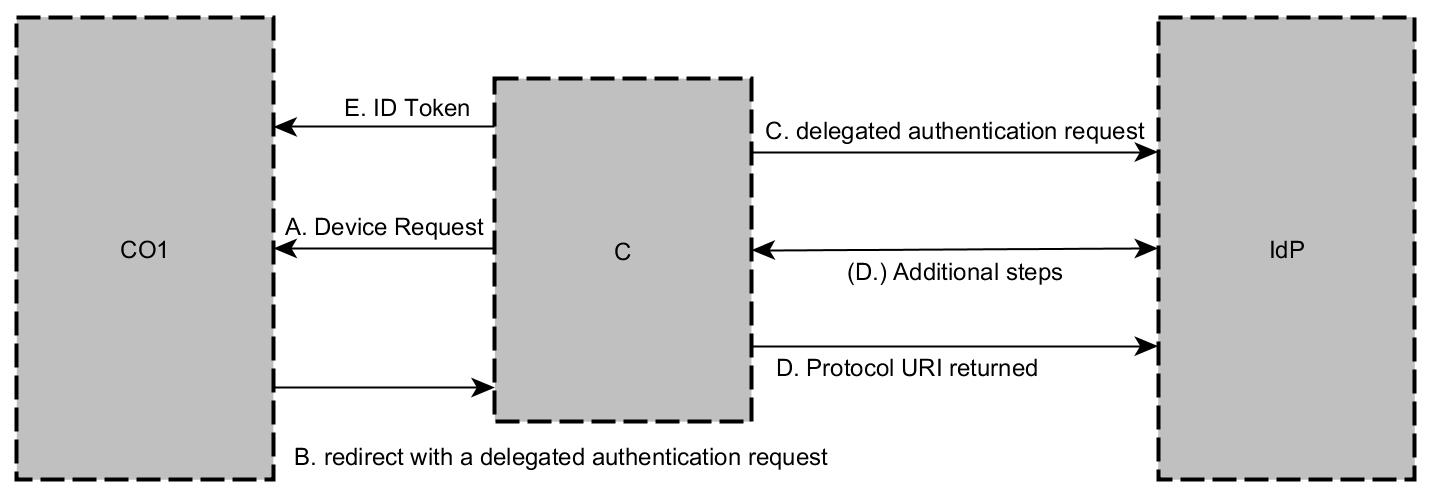
\includegraphics[width=\textwidth]{images/case1}
		\label{fig:example_a}}
	\qquad
	\subfloat[authenticate \& get protocol URI processes][Step 3: authenticate \& get protocol URI processes]{
		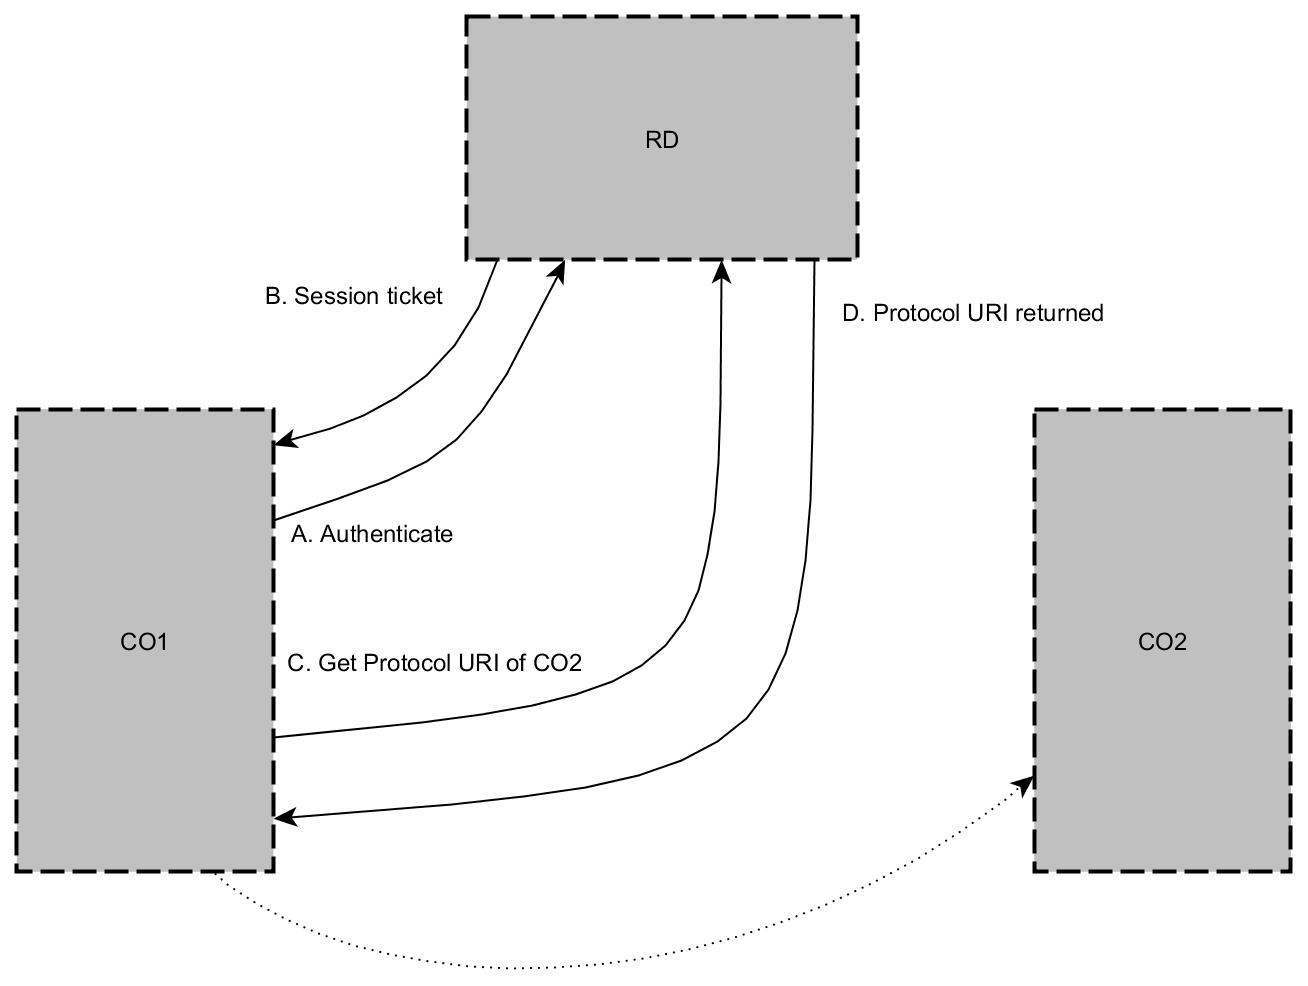
\includegraphics[width=\textwidth]{images/case1_b}
		\label{fig:example_b}}
	\caption{Main steps in the provision of a device crossing domains.}
	\label{fig:example}
\end{figure}

\vspace{1em}
In the process, the only two assumptions made are that every entities trusts the Root Domain (any communication is done over a secure channel, where entities certificates must be validated by the Root Domain certificate) and that the various Operators know how to contact the Root Domain Operator. From those two assumptions, it will later on proved that the design is secure, or at least robust (the zero-risk level doesn't exist in security)\ref{cha:evaluation}.

The possibility to add additional step when authenticating a Principal is also given, as shown in Fig \ref{fig:example_a}. For instance, the IdP could ask the Principal to sign a message with another key. Even sophisticated features like One-Time Passwords (a Consumer would receive a one time code by SMS) could be considered. 

Also, it is assumed that the Principal can send its credentials when redirected from the Client to the IdP. In a normal http environment, the Principal only conveys the message when redirected, but since Websocket redirection are handled on the application layer, this would not be a problem. However, if a Principal forgets to attach the required data, the IdP can request it, thus leading to additional steps.


